% Fork: https://github.com/jamieforth/goldsmiths-phd-thesis-template

% Intended LaTeX compiler: xelatex + biber
% Compile with latexmk should Just Work™
% latexmk -xelatex -shell-escape main.tex

\documentclass[12pt, a4paper]{gsdiss}

\usepackage[a4paper,top=3cm,bottom=3cm,left=4cm,right=3cm]{geometry}

\usepackage{graphicx}           % \includegraphics

% You only need this if you are using SVG images, and it relies on the
% available of external programmes like inkscape.
% \usepackage{svg}                % \includesvg

\usepackage{grffile}            % Allow periods and spaces in graphics
                                % file names.

\usepackage{float}              % Custom floats and the H option.
\usepackage{subfig}             % Combine several figures into one.
\usepackage{wrapfig}            % For figure placement
\usepackage{rotating}           % For sideways figures and tables.

\usepackage{longtable}          % Multipage tables.

\usepackage{fontspec}           % For setting fonts.

\usepackage{csquotes}           % Context sensitive quotations
\usepackage{polyglossia}        % Babel replacement for xelatex
\setmainlanguage[variant=uk]{english}

\usepackage{amssymb}            % Additional maths symbols.
\usepackage{amsthm}             % For theorems etc.

\usepackage{mathtools}          % amsmath plus fixes.
\usepackage{unicode-math}       % Include unicode characters in maths.

\usepackage{algorithmic}        % Typeset pseudo-code.
\usepackage[chapter]{algorithm} % Float algorithmic blocks (e.g. add caption).

% Code formatting: Use either listings or minted to typeset code.
\usepackage{listings}
% Minted requires Python and the Pygments package.
% \usepackage{minted}

\usepackage{url}                % Typeset urls.

\usepackage{paralist}           % Less space in lists.
\let\itemize\compactitem
\let\description\compactdesc
\let\enumerate\compactenum

% Use biblatex+biber for references.
\usepackage[style=authoryear,backend=biber]{biblatex}
\ExecuteBibliographyOptions{
  sorting=nyt,
  maxcitenames=2,
  giveninits=true,
  urldate=long,
  doi=true,
  isbn=false,
  eprint=false,
  uniquename=allinit,
  uniquelist=minyear
}

\addbibresource{refs.bib}

\setmainfont{Libertinus Serif}
\setsansfont{Libertinus Sans}
\setmathfont{Libertinus Math}
% \setmonofont{Libertinus Mono}
\setmonofont{Roboto Mono}

\author{Your name}
\date{\today}
\title{The title}
\supervisor{Dr. A Anon}
%\degree{Doctor of Philosophy}
\degree{BSc Creative Computing}


\usepackage{hyperref}           % For cross references.
\hypersetup{
 pdfauthor={\theauthor},
 pdftitle={\thetitle},
 pdfkeywords={},
 pdfsubject={},
 pdfcreator={},
 pdflang={British},
 colorlinks,
 linkcolor=,
 urlcolor=gray
}

% Custom latex commands.
% Generic notation
\newcommand{\setof}[1]{\ensuremath{\left \{ #1 \right \}}}
\newcommand{\tuple}[1]{\ensuremath{\left \langle #1 \right \rangle }}
\newcommand{\vecb}[1]{\ensuremath{\mathbf{#1}}}
\newcommand{\matb}[1]{\ensuremath{\mathbf{#1}}}
\DeclareMathOperator*{\argmin}{arg\,min}
\DeclareMathOperator*{\argmax}{arg\,max}

% Pattern discovery
\newcommand{\SIA}{\mbox{\texttt{SIA}}}
\newcommand{\SIATEC}{\mbox{\texttt{SIATEC}}}
\newcommand{\COSIATEC}{\mbox{\texttt{COSIATEC}}}

\newcommand{\patternP}{\ensuremath{P}}
\newcommand{\datasetD}{\ensuremath{D}}
%\newcommand{\Pmtp}{\ensuremath{P_{\textsc{mtp}}}}
\newcommand{\Ptec}{\ensuremath{P'}}
\newcommand{\Ptecn}[1]{\ensuremath{\Ptec_{#1}}}
\newcommand{\tec}{\mathcal{T}}
\newcommand{\translator}{\vecb{t}}
\newcommand{\translatorSetT}{\ensuremath{T}} % set of vectors, not
                                % equiv. to familyF

% Cormen set-cover symbols
\newcommand{\setX}{\ensuremath{X}}
\newcommand{\familyF}{\ensuremath{\mathcal{F}}}
\newcommand{\subsetS}{\ensuremath{S}}
\newcommand{\coverC}{\ensuremath{\mathcal{C}}}
\newcommand{\coverCi}{\ensuremath{\mathcal{C}_{i}}}

% SIA functions
\DeclareMathOperator{\fcoverage}{coverage}
\DeclareMathOperator{\fcoveragei}{coverage_{i}}
%\DeclareMathOperator{\funcovered}{uncovered}
\DeclareMathOperator{\fcompressionratio}{compression\;ratio}
\DeclareMathOperator{\fcompactness}{compactness}
\DeclareMathOperator{\fcompactnesssegv}{compactness-v}
\DeclareMathOperator{\fweight}{weight}

\DeclareMathOperator{\fsegment}{\mathit{segment}}
\DeclareMathOperator{\fsegmentv}{\mathit{segment-v}}
\DeclareMathOperator{\fvoice}{\mathit{voice}}
\DeclareMathOperator{\fvoices}{\mathit{voices}}
\DeclareMathOperator{\fstart}{\mathit{start}}
\DeclareMathOperator{\fend}{\mathit{end}}

\newcommand{\heuristic}{h}
\newcommand{\weightW}{W_{\heuristic}}

% Point set symbolic
\newcommand{\sonset}{\ensuremath{\texttt{onset}}}
\newcommand{\smpitch}{\ensuremath{\texttt{mpitch}}}
\newcommand{\svoice}{\ensuremath{\texttt{voice}}}
\newcommand{\scpitch}{\ensuremath{\texttt{cpitch}}}
\newcommand{\sdur}{\ensuremath{\texttt{dur}}}
\newcommand{\scpint}{\ensuremath{\texttt{cpint}}}
\newcommand{\sioi}{\ensuremath{\texttt{ioi}}}

% Function from sym to geo
% \newcommand{\fioi}{\textit{ioi}}
% \newcommand{\fcpint}{\textit{cpint}}


% Point set geometry
\newcommand{\onset}{\ensuremath{\textsc{onset}}}
\newcommand{\cpitch}{\ensuremath{\textsc{cpitch}}}
\newcommand{\dur}{\ensuremath{\textsc{dur}}}
\newcommand{\cpint}{\ensuremath{\textsc{cpint}}}
\newcommand{\ioi}{\ensuremath{\textsc{ioi}}}

\DeclareMathOperator{\fcpitch}{\mathit{cpitch}}
\DeclareMathOperator{\fdur}{\mathit{dur}}

% Symbolic representation of metre
\newcommand{\TMI}{\ensuremath{\mathcal{T}}}
\DeclareMathOperator{\flabel}{\mathit{label}}
\DeclareMathOperator{\froot}{\mathit{root}}
\DeclareMathOperator{\fdepth}{\mathit{depth}}
\DeclareMathOperator{\flevel}{\mathit{level}}
\DeclareMathOperator{\fparent}{\mathit{parent}}
\DeclareMathOperator{\fchildren}{\mathit{children}}
\DeclareMathOperator{\fisleaf}{\mathit{is-leaf}}
\DeclareMathOperator{\fleafnodes}{\mathit{leaf-nodes}}
\DeclareMathOperator{\fchild}{\mathit{child}}
\DeclareMathOperator{\fheight}{\mathit{height}}
\DeclareMathOperator{\farity}{\mathit{arity}}
\DeclareMathOperator{\fposition}{\mathit{position}}

\DeclareMathOperator{\fpioi}{\mathit{p-ioi}}
\DeclareMathOperator{\fonset}{\mathit{onset}}
\DeclareMathOperator{\faenergy}{\mathit{a-energy}}
\DeclareMathOperator{\fcard}{\mathit{cardinality}}
\DeclareMathOperator{\fmeanpioi}{\mathit{mean-p-ioi}}
\DeclareMathOperator{\fmeanaenergy}{\mathit{mean-a-energy}}

% Conceptual spaces
\newcommand{\metrep}{\textsc{\mbox{metre-p}}}
\newcommand{\metres}{\textsc{\mbox{metre-s}}}
\newcommand{\tempo}{\textsc{\mbox{tempo}}}
\newcommand{\meanPulseIOI}[1]{\ensuremath{\textsc{mean\_p\_ioi}^{#1}}}
\newcommand{\meanAttEnergy}[1]{\ensuremath{\textsc{mean\_a\_energy}^{#1}}}
\newcommand{\cratio}[1]{\ensuremath{\textsc{c\_ratio}^{#1}}}

\newcommand{\pulseIOI}[1]{\ensuremath{\textsc{p\_ioi}^{#1}}}
\newcommand{\attEnergy}[1]{\ensuremath{\textsc{a\_energy}^{#1}}}

\newcommand{\nnk}[1]{\ensuremath{k\text{#1}}}
\newcommand{\mathkequals}[1]{\ensuremath{k\text{~=~#1}}}
\newcommand{\mathnequals}[1]{\ensuremath{n\text{~=~#1}}}

% Algorithms
\DeclareMathOperator{\mapTreeMeanPulseIOI}{\mathtt{MAP\_T\_MEAN\_PIOI}}
\DeclareMathOperator{\mapTreeMeanEnergy}{\mathtt{MAP\_T\_MEAN\_AENERGY}}
\DeclareMathOperator{\mapTreeCRatio}{\mathtt{MAP\_T\_MEAN\_CRATIO}}

\DeclareMathOperator{\mapTreePulseIOI}{\mathtt{MAP\_T\_PIOI}}
%\DeclareMathOperator{\fabsDepthOffset}{\mathtt{ABS\_CYCLE\_DEPTH\_OFFSET}}
\DeclareMathOperator{\fabsDepthOffset}{\mathit{abs-depth-offset}}
%\DeclareMathOperator{\fwithinCycleOffset}{\mathtt{WITHIN\_CYCLE\_NODE\_OFFSET}}
\DeclareMathOperator{\fwithinCycleOffset}{\mathit{within-cycle-offset}}
\DeclareMathOperator{\fillIOIDomain}{\mathtt{FILL\_PIOI\_DOMAIN}}
\DeclareMathOperator{\repeatSubSeq}{\mathtt{REPEAT\_SUB\_SEQ}}
\DeclareMathOperator{\mapTreeAttEnergy}{\mathtt{MAP\_T\_AENERGY}}
\DeclareMathOperator{\fabsWithinNCycleOffset}{\mathit{abs-within-n-cycle-offset}}


% Custom title page.
\renewcommand\maketitle{
  \begin{titlepage}
    \clearpage
    \fancyhf{}
    \rhead{
      
\includegraphics[width=50mm]{images/goldsmiths-logo-pantone-442.pdf}
    }
    \renewcommand{\headrulewidth}{0pt}

    \thispagestyle{fancyplain}
    \begin{center}
      \vspace*{1.5in}
      \noindent\begin{minipage}[t]{.85\textwidth}
        \centering\large

        {\LARGE \thetitle}
      \end{minipage}

      \par
      \vspace{1.0in}
      {\large \theauthor}

      \vfill

      \ifdef{\thesupervisor}{\large Supervisor: \thesupervisor}

      \par
      \vspace{1.0in}
      Submitted in partial fulfilment of the requirements\\
      for the degree of \thedegree\\
      of the
      University of London.
      \par
      \vspace{0.25in}
      Department of Computing
      \par
      Goldsmiths, University of London
      \par
      \vspace{0.5in}
      \thedate
    \end{center}
  \end{titlepage}

  \clearpage
  \vspace*{\stretch{2}}
  \begin{center}
    \begin{minipage}{0.7\textwidth}
      \noindent I certify that this dissertation, and the research to which
      it refers, are the result of my own work.
    \end{minipage}
  \end{center}
  \vspace{\stretch{3}}
  \clearpage
}


\begin{document}

\maketitle

\chapter*{Abstract}

Aim for around 200–300 words to highlight the main points and
contributions of your project.

\chapter*{Acknowledgements}

% \chapter*{Licence}

This work is copyright \copyright \ 2016 Your Name, and is licensed
under TO BE DECIDED - CHOOSE YOUR OWN OR USE CUURENT UNIVERSITY
GUIDELINES the Creative Commons Attribution-Share Alike 3.0 Unported
Licence. To view a copy of this licence, visit \\
\url{http://creativecommons.org/licenses/by-sa/3.0/} \\
or send a letter to Creative Commons, 171 Second Street, Suite 300,
San Francisco, California, 94105, USA.

\begin{center}

%	\includegraphics [width =1cm]  {images/cc}
%	\includegraphics [width =1cm]  {images/by}
%	\includegraphics [width =1cm]  {images/sa}

\end{center}

% \chapter*{Related Publications}

Portions of the work detailed in this dissertation have appeared in
the following publications. \\[1ex]

\noindent An earlier version of the research reported in chapter
\ref{ch:evaluation} was also reported in:

\fullcite{foo2017} \\[1ex]


\tableofcontents
\listoftables
\listoffigures
\chapter*{List of abbreviations}

\begin{table}[htbp]
  \begin{center}
    \begin{tabular}{ll}

      XXX &	something \\

    \end{tabular}
  \end{center}
\end{table}


% Chapters

\chapter{Introduction}
\label{ch:intro}

% Choose your own headings.

\section{Motivation}



\section{Aim}



\section{Thesis structure}


\begin{description}
%\item[Chapter \ref{ch:background}]
%\item[Chapter \ref{ch:evaluation}]
\item[Chapter \ref{ch:conclusions}]
\end{description}


\section{Contributions}
Contributions of this thesis are:
\begin{itemize}
\item Blah %\ref{ch:}
\end{itemize}

\chapter{Background}
\label{ch:background}

% Choose your own headings.

\section{Background}

\section{Literature review}

\textcite{foo2017} propose…

%%% Local Variables:
%%% mode: latex
%%% TeX-master: "../../main"
%%% End:

\chapter{Specification and design}
\label{ch:specification}

% Choose your own headings.

\section{System design}

Diagrams would be good here.

%%% Local Variables:
%%% mode: latex
%%% TeX-master: "../../main"
%%% End:

\chapter{Implementation}
\label{ch:implementation}

% Choose your own headings.

\section{System architecture}

\section{Software implementation}

Only include code where it is essential to make a point, e.g. a clever
optimisation trick you implemented. Do not copy and paste lots of
boilerplate code in your report, refer to your git repository.

\begin{lstlisting}[caption={Example of typesetting code with
    \texttt{listing}. Keep code snippets short!}]
# Generate example data.
np.random.seed(13)              # Seed the random number generator.
n=50                            # Number of observations.
happiness_levels = ['very sad', 'sad', 'neutral', 'happy',
                    'very happy']
happiness_prob = [0.05, 0.2, 0.3, 0.35, 0.1]

s = pd.Series(np.random.choice(happiness_levels, n,
                               p=happiness_prob),
              name='happiness')

# Set correct data type.
s = s.astype(
    pd.api.types.CategoricalDtype(
        ordered=True,
        categories=happiness_levels))

# Compute percentages.
pc = s.value_counts(sort=False, normalize=True) * 100

# Plot.
ax = pc.plot.bar(rot=0)
ax.yaxis.set_major_formatter(
    mpl.ticker.PercentFormatter(decimals=0))
ax.set_xlabel('happiness raitings')

plt.show()
\end{lstlisting}


% \begin{listing}[H]
% \begin{minted}[numbers=left,python3]{python}
% # Generate example data.
% np.random.seed(13)              # Seed the random number generator.
% n=50                            # Number of observations.
% happiness_levels = ['very sad', 'sad', 'neutral', 'happy',
%                     'very happy']
% happiness_prob = [0.05, 0.2, 0.3, 0.35, 0.1]

% s = pd.Series(np.random.choice(happiness_levels, n,
%                                p=happiness_prob),
%               name='happiness')

% # Set correct data type.
% s = s.astype(
%     pd.api.types.CategoricalDtype(
%         ordered=True,
%         categories=happiness_levels))

% # Compute percentages.
% pc = s.value_counts(sort=False, normalize=True) * 100

% # Plot.
% ax = pc.plot.bar(rot=0)
% ax.yaxis.set_major_formatter(
%     mpl.ticker.PercentFormatter(decimals=0))
% ax.set_xlabel('happiness raitings')

% plt.show()
% \end{minted}
% \caption{Example of typesetting code with \texttt{minted}. Keep code snippets short!}
% \end{listing}

%%% Local Variables:
%%% mode: latex
%%% TeX-master: "../../main"
%%% End:

\chapter{Software testing}
\label{ch:testing}

% Choose your own headings.

\section{Unit testing}

\subsection{Results}

\begin{table}[H]
\caption{This is some example data}
\centering
\begin{tabular}{rrr}
\toprule
id & a & b\\
\midrule
0 & 1 & 2\\
1 & 3 & 4\\
\midrule
total & 4 & 6\\
\bottomrule
\end{tabular}
\end{table}

\section{Load testing}

\subsection{Results}

%%% Local Variables:
%%% mode: latex
%%% TeX-master: "../../main"
%%% End:

\chapter{Evaluation}
\label{ch:evaluation}

% Choose your own headings.

\section{User testing}

\section{Results}

Figure~\ref{fig:user-ratings} shows…

\begin{figure}[H]
\centering
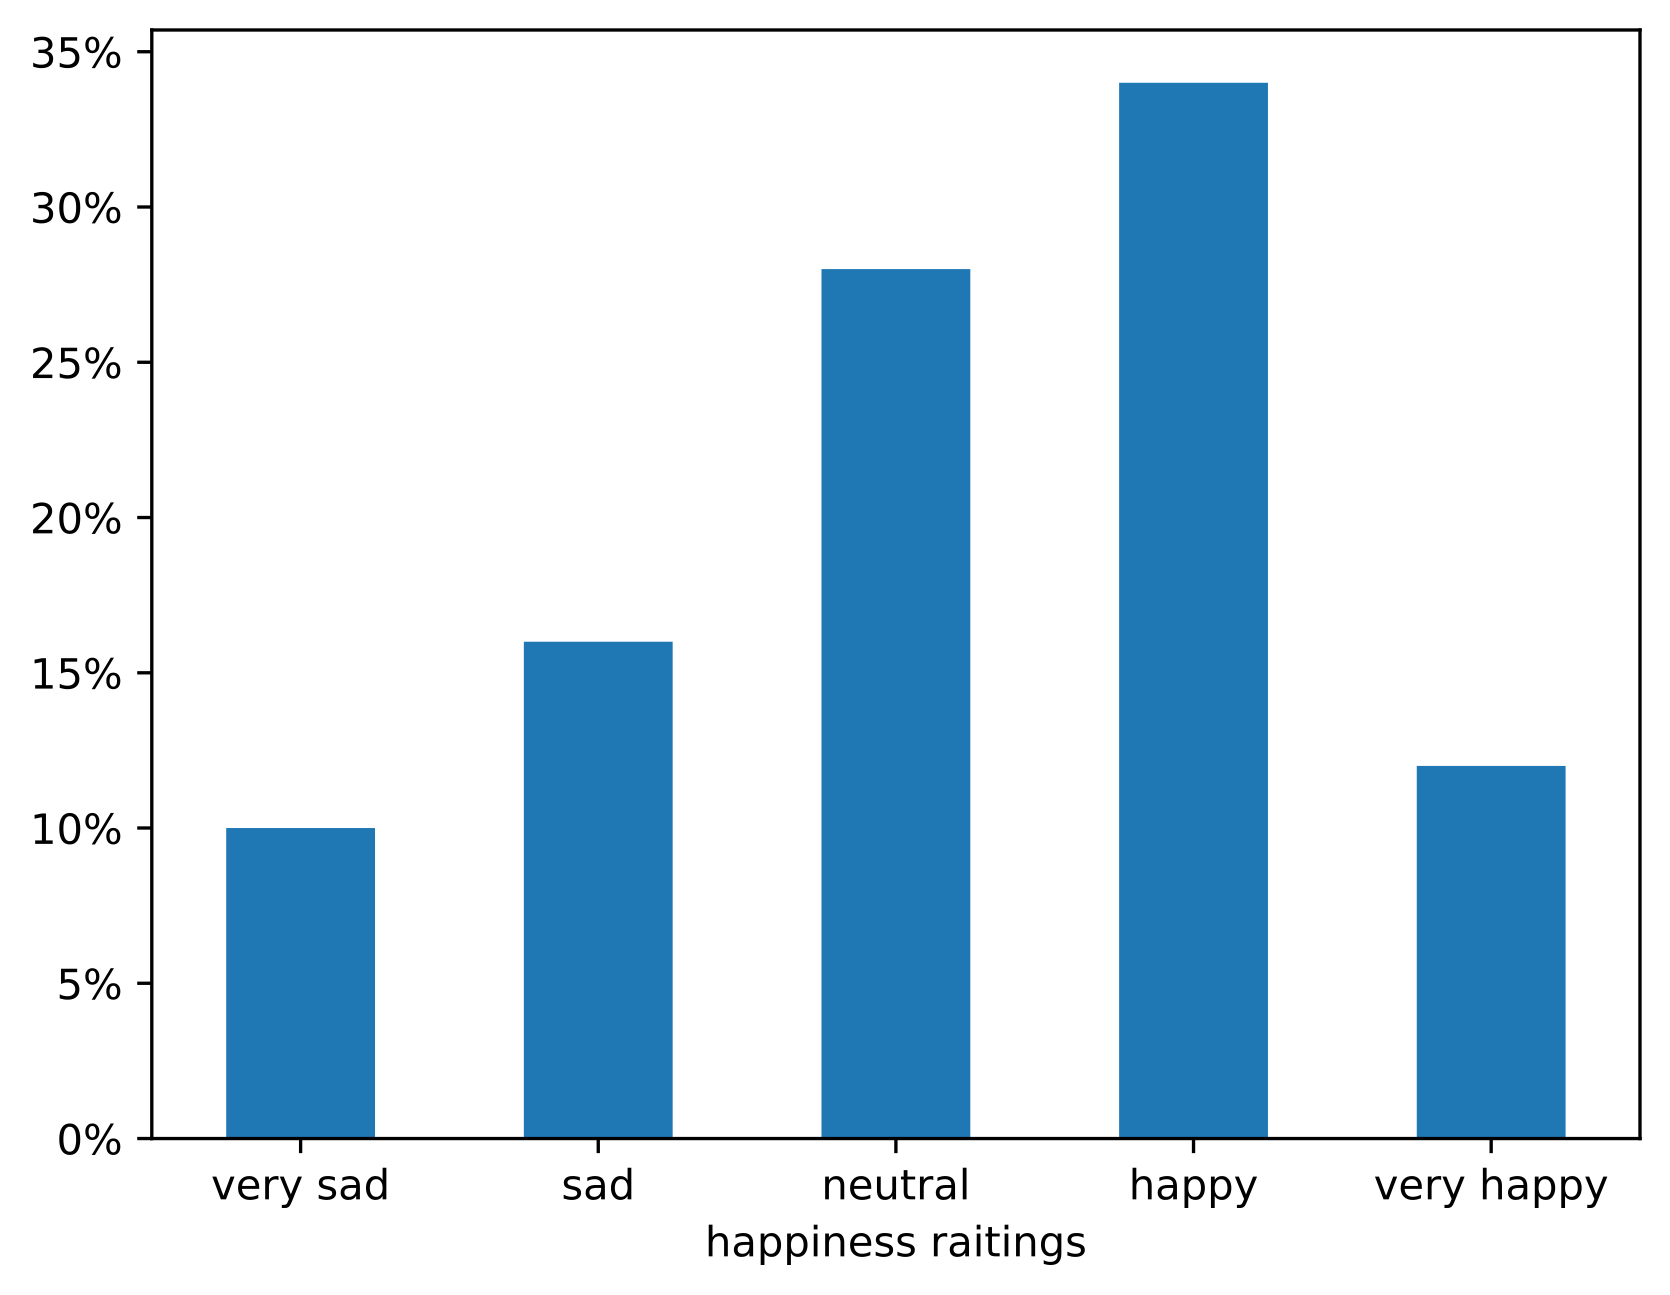
\includegraphics[width=.9\linewidth]{./figures/05-user-results}
% \includesvg[width=.9\linewidth]{./figures/05-user-results}
\caption{User ratings}
\label{fig:user-ratings}
\end{figure}

%%% Local Variables:
%%% mode: latex
%%% TeX-master: "../../main"
%%% End:

\chapter{Conclusions and further work}
\label{ch:conclusions}

\section{Summary of contributions}

\section{Further work}

%%% Local Variables:
%%% mode: latex
%%% TeX-master: "../../main"
%%% End:


% References

\printbibliography

% Appendices

\appendix
\chapter{Notational conventions}
\label{sec:notation}

\begin{center}
  \begin{tabu}{ll}
    \(S=\setof{\ldots}\) & the set \(S\)\\
    \(S \times S'\) & the Cartesian product of \(S\) and \(S'\)\\
    \(\rvert S \rvert\) & the cardinality of \(S\)\\
    \(\emptyset\) & the empty set\\
                         & \\
    \(\mathbb{R}\) & real numbers\\
    \(\mathbb{R^+}\) & positive real numbers\\
    \(\mathbb{R}^k\) & \nnk{-dimensional} real vector space\\
    \(\mathbb{Z}\) & integer numbers\\
    \(\mathbb{Z^+}\) & positive integer numbers\\
    \(\mathbb{N}\) & non-negative integer numbers\\
    \([x,y]\) & inclusive real-number interval between \(x\) and \(y\)\\
    \([x..y]\) & inclusive integer-number interval between \(x\) and \(y\)\\
                         & \\
    \(\vecb{v}=\tuple{\ldots}\) & the vector \(\vecb{v}\)\\
    \(\matb{M} = [m_{ij}]\) & the matrix \(\matb{M}\)\\
    \(\vecb{m}_i^j =\tuple{e_1, e_2, \ldots, e_j}\) & the ordered sequence of length \(j \in \mathbb{Z}^+\), indexed by \(i \le j\)\\
    \(\Vert\) & tuple concatenation: \(\tuple{0,1} \Vert \tuple{2,3} \to \tuple{0,1,2,3}\)\\
    \(\top\) & the symbol denoting undefined\\
  \end{tabu}
\end{center}


\end{document}
